 \iffalse
\let\negmedspace\undefined
\let\negthickspace\undefined
\documentclass[journal,12pt,twocolumn]{IEEEtran}
\usepackage{cite}
\usepackage{amsmath,amssymb,amsfonts,amsthm}
\usepackage{algorithmic}
\usepackage{graphicx}
\usepackage{textcomp}
\usepackage{xcolor}
\usepackage{txfonts}
\usepackage{listings}
\usepackage{enumitem}
\usepackage{mathtools}
\usepackage{gensymb}
\usepackage{comment}
\usepackage[breaklinks=true]{hyperref}
\usepackage{tkz-euclide} 
\usepackage{listings}
\usepackage{gvv}                                        
\def\inputGnumericTable{}                                 
\usepackage[latin1]{inputenc}                                
\usepackage{color}                                            
\usepackage{array}                                            
\usepackage{longtable}                                       
\usepackage{calc}                                             
\usepackage{multirow}                                         
\usepackage{hhline}                                           
\usepackage{ifthen}                                           
\usepackage{lscape}
\usepackage{caption}
\newtheorem{theorem}{Theorem}[section]
\newtheorem{problem}{Problem}
\newtheorem{proposition}{Proposition}[section]
\newtheorem{lemma}{Lemma}[section]
\newtheorem{corollary}[theorem]{Corollary}
\newtheorem{example}{Example}[section]
\newtheorem{definition}[problem]{Definition}
\newcommand{\BEQA}{\begin{eqnarray}}
\newcommand{\EEQA}{\end{eqnarray}}
\newcommand{\define}{\stackrel{\triangle}{=}}
\theoremstyle{remark}
\newtheorem{rem}{Remark}
\begin{document}
\parindent 0px
\bibliographystyle{IEEEtran}
\vspace{3cm}

\title{NCERT 11.14 12Q}
\author{EE23BTECH11012 - Chavan Dinesh$^{*}$% <-this % stops a space
}
\maketitle
\newpage
\bigskip

\renewcommand{\thefigure}{\arabic{figure}}
\renewcommand{\thetable}{\arabic{table}}
\large\textbf{\textsl{Question:}}
Plot the corresponding reference circle for each of the following simple harmonic
motions. Indicate the initial (t = 0) position of the particle, the radius of the circle,and the angular speed of the rotating particle. For simplicity, the sense of rotation
may be fixed to be anticlockwise in every case: ($x$ is in cm and $t$ is in $s$)
\begin{enumerate}[label=\alph*)]
    \item $x = -2 \sin(3t + \frac{\pi}{3})$
    \item $x = \cos(\frac{\pi}{6} - t)$
    \item $x = 3 \sin(2\pi t + \frac{\pi}{4})$
    \item $x = 2 \cos(\pi t)$
\end{enumerate}

\solution
\fi
\begin{table}[htbp]
    \centering
    \setlength{\extrarowheight}{5pt}
      \begin{tabular}{|c|c|c|c|c|}
        \hline
        \textbf{S.No} & \textbf{$f$(in Hz)} &\textbf{$A$(in cm)}&\textbf{$\phi$}\\
        \hline
        $1.$ & $\frac{3}{2\pi}$&$2$ & $\frac{5\pi}{6}$\\
         \hline
        $2.$ & $\frac{1}{2\pi}$ &$1$&$\frac{-\pi}{6}$\\
        \hline
        $3.$ & $1$ & $3$&$\frac{3\pi}{4}$\\
        \hline
        $4.$ & $\frac{1}{2}$ & $1$&$0$\\
        \hline
    \end{tabular}
 

    \caption{Input table}
    \label{tab:parameter_table.11.14.12.analog}
\end{table}
\begin{enumerate}[label=\roman*)]
\item \begin{align}
    x = -2 \sin\left(3t + \frac{\pi}{3}\right)\\
   x =2\cos\left(3t+\frac{5\pi}{6}\right)
\end{align}
\begin{figure}[!htbp]
    
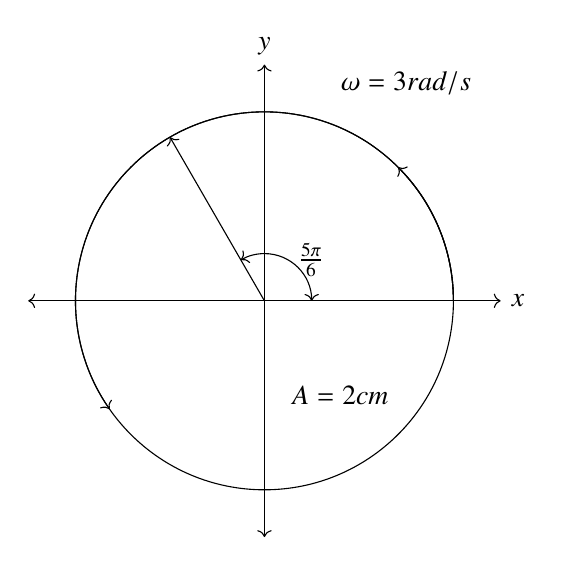
\begin{tikzpicture}[scale=1.2]
    % Axis
    \draw[<->] (-2.5,0) -- (2.5,0) node[right] {$x$};
    \draw[<->] (0,-2.5) -- (0,2.5) node[above] {$y$};
    \draw (0,0) circle (2);
     % \node at ({-2*cos(120)}, {2*sin(120)}) {$<$};
     \draw[->] (2,0) arc (0:45:2);
     \draw[->] (2,0) arc (0:215:2);

    \draw[->] (0,0) -- (120:2);
    \draw[<->] (0.5,0) arc (0:120:0.5) node[midway, right] {$\frac{5\pi}{6}$};
    \node at (1.5,2.3) {$\omega = 3 rad/s$};
    \node at (0.8,-1) {$A =2cm$};
    
\end{tikzpicture}


\end{figure}
\item \begin{align}
    x = \cos\left(\frac{\pi}{6} - t\right)
\end{align}
\begin{figure}[!htbp]
    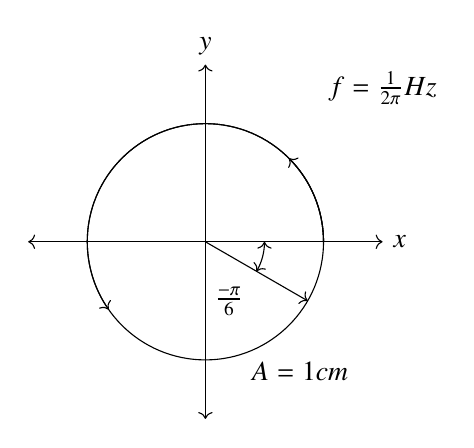
\begin{tikzpicture}[scale=1.5]
\centering
    % Axis
    \draw[<->] (-1.5,0) -- (1.5,0) node[right] {$x$};
    \draw[<->] (0,-1.5) -- (0,1.5) node[above] {$y$};
    \draw (0,0) circle (1);
     % \node at ({-2*cos(120)}, {2*sin(120)}) {$<$};
     \draw[->] (1,0) arc (0:45:1);
     \draw[->] (1,0) arc (0:215:1);

    \draw[->] (0,0) -- (330:1);
    \draw[<->] (0.5,0) arc (0:-30:0.5) node at (0.2,-0.5){$\frac{-\pi}{6}$};
    \node at (1.5,1.3) {$f = \frac{1}{2\pi}Hz$};
    \node at (0.8,-1.1) {$A =1cm$};
\end{tikzpicture}

\end{figure}

\item \begin{align}
    x &= 3 \sin\left(2\pi t + \frac{\pi}{4}\right)\\
    x &= -3\cos\left(2\pi t + \frac{3\pi}{4}\right)
\end{align}
\begin{figure}[!htbp]
    \begin{tikzpicture}[scale=1]
\centering
    % Axis
    \draw[<->] (-3.5,0) -- (3.5,0) node[right] {$x$};
    \draw[<->] (0,-3.5) -- (0,3.5) node[above] {$y$};
    \draw (0,0) circle (3);
     % \node at ({-2*cos(120)}, {2*sin(120)}) {$<$};
     \draw[->] (3,0) arc (0:45:3);
     \draw[->] (3,0) arc (0:215:3);

    \draw[->] (0,0) -- (315:3);
    \draw[<->] (0.5,-0.5) arc (-45:-180:0.707) node at (-0.9,-1){$\frac{3\pi}{4}$};
    \node at (1.5,1.3) {$\omega = 2\pi rad/s$};
    \node at (1.8,-0.5) {$A =1cm$};
\end{tikzpicture}

\end{figure}

\item 
\begin{align}
    x = 2 \cos(\pi t)
\end{align}
\begin{figure}[!htbp]
    \begin{tikzpicture}[scale=1.2]
\centering
    % Axis
    \draw[<->] (-2.5,0) -- (2.5,0) node[right] {$x$};
    \draw[<->] (0,-2.5) -- (0,2.5) node[above] {$y$};
    \draw (0,0) circle (2);
     % \node at ({-2*cos(120)}, {2*sin(120)}) {$<$};
     \draw[->] (2,0) arc (0:45:2);
      \draw[->] (2,0) arc (0:215:2);

    \node at (2.2,1.8) {$\omega = \pi rad/s$};
    \node at (0.9,-0.6) {$A =2cm$};
\end{tikzpicture}

\end{figure}

\end{enumerate}

\begin{figure}[ht]
    \centering
    \includegraphics[width = \columnwidth]{ncert-physics/11/14/12/figs/Figure_1.png}
    \caption{}
\end{figure}

\begin{figure}[ht]
    \centering
    \includegraphics[width = \columnwidth]{ncert-physics/11/14/12/figs/Figure_2.png}
    \caption{}
\end{figure}

\begin{figure}[ht]
    \centering
    \includegraphics[width = \columnwidth]{ncert-physics/11/14/12/figs/Figure_3.png}
    \caption{}
\end{figure}

\begin{figure}[ht]
    \centering
    \includegraphics[width = \columnwidth]{ncert-physics/11/14/12/figs/Figure_4.png}
    \caption{}
\end{figure}
